



\subsection{Calibrating the Cohesive Energies}

The experimental cohesive energies for \acrshort{bcc} Iron, \acrshort{fcc} Palladium and \acrshort{hcp} Ruthenium are know and these could be used in the reference database.  However, forcing the \acrshort{dft} data to the experimental values has an issue as there is likely to be an error between the computed cohesive energy.  If the difference between the computed relaxed and isolated atom energies is less than the experimental cohesive energy, the potential functions would tend towards an energy less than zero as atoms move apart becoming isolated.  If the computed energy difference is great, then the potential would have positive energy isolated atoms.  

\begin{figure}[h]
\begin{center}
\includegraphics[width=0.5\linewidth]{chapters/results_dft_reference_db/isolated/isolated_63.eps}
\caption{Isolated atom energies as cell size increase}
\label{fig:isolatedatoms}
\end{center}
\end{figure}

Rather than use the experimental values, and either accept the errors or try to scale the \acrshort{dft} energies, forces and stresses, only the computed values will be used to make up the configuration database.

\begin{table}[h]
\begin{center}
\begin{tabular}{c c c c c}
\hline\hline
Element & Structure & Isolated Energy (Ry) & Relaxed Energy (Ry) & Cohesive Energy (eV) \\
\hline\hline
Fe      & BCC       & -4474.99115          & -4479.83524         & 4.84 (exp. 4.32)\\
Fe      & FCC       & -4474.99115          & -4479.78095         & 4.79 \\
Pd      & FCC       & -6962.47261          & -6966.52234         & 4.05 (exp. 3.91)\\
Ru      & HCP       & -5866.39894          & -5873.22666         & 6.83 (exp. 6.74)\\
Ru      & FCC       & -5866.39894          & -5873.11029         & 6.71 \\
\hline\hline
\end{tabular}
\end{center}
\caption{\acrshort{dft} calculated energies per atom}
\label{table:calculatedcohesiveenergies}
\end{table}

The errors on the cohesive energies for Pd, Ru and Fe are approximately 1\%, 4\% and 12\% respectively.  These isolated energies will be used to adjust all other energies computed in this reference database.


\subsection{Cohesive Energy Plots}

The cohesive energy was investigated by applying an orthorhombic strain to the regular lattice until the change in energy dropped appreciably.  This helps to compute the cohesive energy using \acrshort{dft} but also provides a set of configurations with energies and stresses that form part of the  







\subsection{Surface Energy}

The surface energy of each was only calculated in the (1,0,0) plane.  Rather than just compute the value of the surface energy only, the bulk was split along the (1,0,0) plane and the separation between the surfaces was increased in steps until the change in energy dropped.  A \acrshort{scf} calculation was computed for each step as well as an atom relaxed computation to arrange the atoms in their most optimal position.

\begin{figure}[h]
\begin{center}
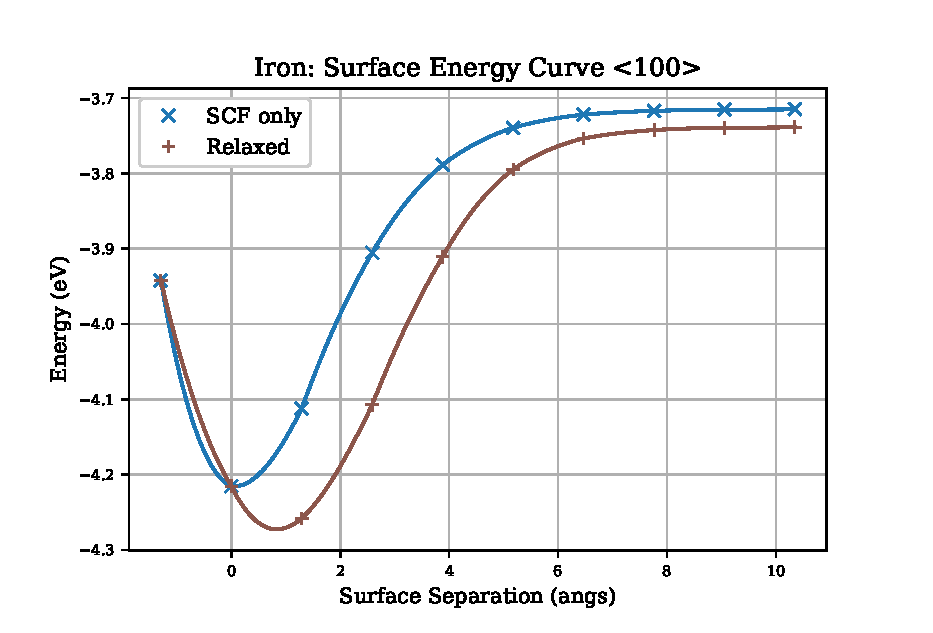
\includegraphics[width=0.5\linewidth]{chapters/results_dft_reference_db/plots/fe/fe_surface_energy.eps}
\caption{Surface energy calculations for FCC Iron}
\label{fig:ironsurfaceenergy}
\end{center}
\end{figure}

In the case of Iron there is a marked difference between the relaxed and non-relaxed calculations.  At one point the atoms find a more favourable position than the computed relaxed FCC positions.  This isn't too surprising as under normal conditions \acrshort{fcc} is not the stable state of iron, \acrshort{bcc} is with a cohesive energy of $-4.316$eV.  The curve plotted doesn't drop below $-4.3$eV.

\begin{figure}[h]
\begin{center}
\includegraphics[width=0.5\linewidth]{chapters/results_dft_reference_db/defects/fe_slab.png}
\caption{Effect of randomly perturbing atom locations}
\label{fig:ironsurfaceenergy}
\end{center}
\end{figure}

The spin of the iron atoms in the calculation are aligned along the z-axis, parallel and anti-parallel to the slab.  Due to time constraints other slab directions and larger bulk configurations with 108 or 256 atoms were not investigated.  The area of the surface is square, and with a lattice parameter of $3.42$ angstrom, the 2x2x2 cell gives the surface an area of $46.845 \text{ angstrom}^2$.  The difference in energy between the atoms in bulk and in the slab is $15.249$eV which gives a surface energy of $1.628 \times 10^{-1} \text{eV}/\text{ang}^{2}$ ($2.608 \times 10^3 \text{mJ}/\text{m}^2$, equivalent units to $\text{erg}/\text{cm}^{2}$).  Whilst there isn't an experimental value for \acrshort{fcc} Iron, the surface energy for \acrshort{bcc} Iron has been measured to be $2.525 \times 10^{3} \text{erg}/\text{cm}^{2}$\cite{ironsurfaceenergy}.

\begin{figure}[h]
\begin{center}
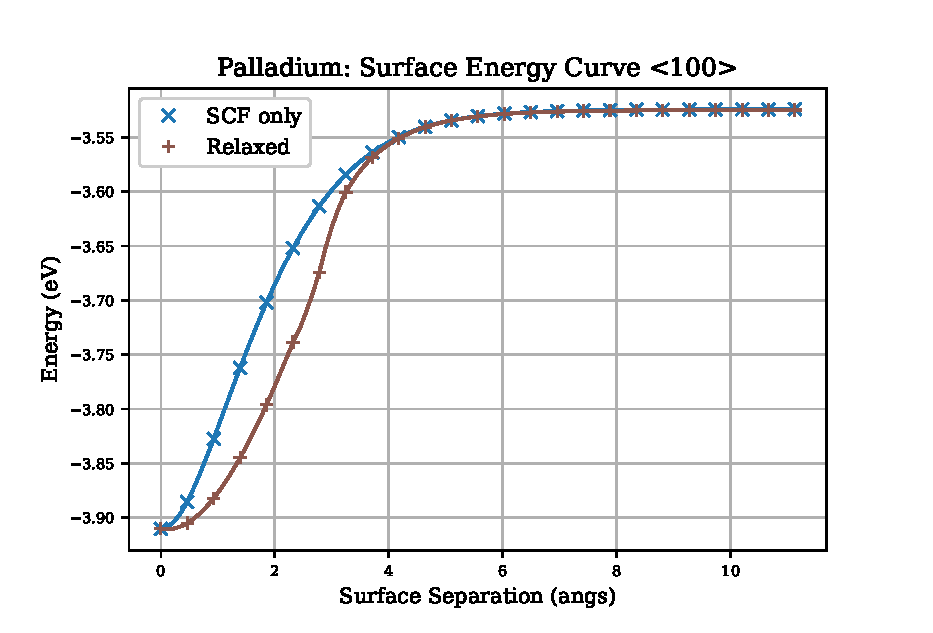
\includegraphics[width=0.5\linewidth]{chapters/results_dft_reference_db/plots/pd/pd_surface_energy.eps}
\caption{Surface energy calculations for FCC Palladium}
\label{fig:pdsurfaceenergy}
\end{center}
\end{figure}

The Palladium calculations were non magnetic, although the y-axis was used as that perpendicular to the slab.  The energy difference between the slab and bulk is $12.327$eV and the 2x2x2 cell, with a lattice parameter of $3.93$ angstrom there is a surface area of $61.623 \text{angstrom}^2$.  The calculated surface energy as a result is $1.602 \times 10^3 \text{mJ}/\text{m}^2$.  Previous work has estimated the surface energies to be $2.000 \times 10^3 \text{mJ}/\text{m}^2$\cite{pdsurfaceenergy},  $1.850 \times 10^3 \text{mJ}/\text{m}^2$\cite{pdsurfaceenergy},  $1.844 \times 10^3 \text{mJ}/\text{m}^2$\cite{pdsurfaceenergy} and $1.645 \times 10^3 \text{mJ}/\text{m}^2$\cite{shengeamonline}.


\begin{figure}[h]
\begin{center}
\includegraphics[width=0.5\linewidth]{chapters/results_dft_reference_db/plots/ru/ru_surface_energy.eps}
\caption{Surface energy calculations for FCC Ruthenium}
\label{fig:rusurfaceenergy}
\end{center}
\end{figure}




\subsection{Defects}





\subsection{Configurations with Randomised Positions}





\begin{comment}
%%%%%%%%%%%%%%%%%%%%%%%%%%%%%%%%%%%%%%%%%%%%%%%%%%%%%%%%%%%%%%%%%%%%%%%%%%%%%%%%%%%%%%%%%%%%%%%%%%%%%%%%%%
%%
%%  QEFORFIT
%%  
%%%%%%%%%%%%%%%%%%%%%%%%%%%%%%%%%%%%%%%%%%%%%%%%%%%%%%%%%%%%%%%%%%%%%%%%%%%%%%%%%%%%%%%%%%%%%%%%%%%%%%%%%%

\FloatBarrier
\section{QEFORFIT Python Code}


A program was created in Python that generates input files for PWscf.  The user specifies a template file then parameters such as the crystal type, lattice parameters, defects, interstitials and vacancies.  The user may choose whether or not the atoms should be moved from their perfect crystal location by a small amount and whether the lattice parameter should be varied.  The program then creates the user specified number of input files for PWscf. 

\subsection{Source Code and Instructions}

The source code and instructions on how to use the program are available to download from GitHub.

https://github.com/BenPalmer1983/qeforfit

\FloatBarrier

\subsection{Gaussian Random Distribution}

The positions of the atoms are moved from the perfect crystal locations by a random amount.  The minimum and maximum amount to be moved is specified by the user, and a random value between these is selected.  The distribution is not flat but takes the shape of a Gaussian curve (fig \ref{fig:gheatdistribution}), so there is less chance that the atom will be moved to either extreme.

\begin{figure}
\centering
\begin{minipage}{.80\textwidth}
\centering
\includegraphics[width=.9\linewidth]{chapters/results_dft_reference_db/images/gheat-distribution.eps}
\caption{Gheat distribution function}
\label{fig:gheatdistribution}
\end{minipage}

\begin{minipage}{.80\textwidth}
\centering
\includegraphics[width=.9\linewidth]{chapters/results_dft_reference_db/images/temperatureplot.eps}
\caption{Maximum displacement from perfect crystal position against the increase in temperature of the system}
\label{fig:gheattemperatureplot}
\end{minipage}
\end{figure}

The Gaussian randomisation class is detailed in the appendix (\ref{chapter:appendix-qeforfit}).  As the atoms are perturbed further and further, the energy and therefore temperature of the system increases.  This may change depending on the element and crystal structure, but a maximum displacement for aluminium atoms of 0.1 angstrom increases the energy and temperature to approximately 40K (fig. \ref{fig:gheattemperatureplot}).

\FloatBarrier

\subsection{DFT Configuration Database}

The QEFORFIT code was used to create files that contributed towards the DFT configuration database.  The broken symmetry caused by the random perturbation of atoms in the configurations caused the calculation to take a long time to complete.  The calculations were also very resource intensive, using up to 100GB of RAM and 20-40 cores for up to a day per configuration.

In addition to this, quite often the SCF convergence would either fail, or complete the maximum number of iterations (which was set high, at 100) without converging, which would also be considered a fail (listing \ref{list:sampleresources}).

\begin{lstlisting}[style=sPseudo,caption={Sample output file to show resource usage and sample error codes},label={list:sampleresources}]
--------------------------------------------------------------------------
WARNING: There was an error initializing an OpenFabrics device.

  Local host:   bear-pg0211u07a
  Local device: mlx5_0
--------------------------------------------------------------------------

     Program PWSCF v.6.3 starts on 10Nov2020 at  7:58:30 

     This program is part of the open-source Quantum ESPRESSO suite
     for quantum simulation of materials; please cite
         "P. Giannozzi et al., J. Phys.:Condens. Matter 21 395502 (2009);
         "P. Giannozzi et al., J. Phys.:Condens. Matter 29 465901 (2017);
          URL http://www.quantum-espresso.org", 
     in publications or presentations arising from this work. More details at
     http://www.quantum-espresso.org/quote

     Parallel version (MPI & OpenMP), running on      40 processor cores
     Number of MPI processes:                40
     Threads/MPI process:                     1

     MPI processes distributed on     1 nodes
     R & G space division:  proc/nbgrp/npool/nimage =      40

     ---

     Estimated max dynamical RAM per process >       2.11 GB

     Estimated total dynamical RAM >      84.34 GB
     Generating pointlists ...

     ---

     Writing output data file zDmzKgmzhrarwYka.save/
-------------------------------------------------------
Primary job  terminated normally, but 1 process returned
a non-zero exit code.. Per user-direction, the job has been aborted.
-------------------------------------------------------
--------------------------------------------------------------------------
mpirun detected that one or more processes exited with non-zero status, thus causing
the job to be terminated. The first process to do so was:

  Process name: [[18842,1],0]
  Exit code:    38
--------------------------------------------------------------------------
\end{lstlisting}

Due to the large amount of resources required and the regular failure to converged, there were a reduced number of configurations: 1 for Iron, 2 for Iron-Palladium, 10 for Palladium (list. \ref{list:sampleresources}).  

The Iron and Palladium PWscf output files produced by the QEEOS code, that were used to calculate the equation of state and elastic constants, were added to the database of files, giving a total of 154 configurations for the Iron-Palladium potential fitting.
\end{comment}




